
% Load the kaobook class
\documentclass[
	fontsize=10pt, % Base font size
	twoside=false, % Use different layouts for even and odd pages (in particular, if twoside=true, the margin column will be always on the outside)
	%open=any, % If twoside=true, uncomment this to force new chapters to start on any page, not only on right (odd) pages
%%	secnumdepth=1, % How deep to number headings. Defaults to 1 (sections)
]{kaobook}

\newcommand{\discipline}{Sciences Industrielles de l'Ingénieur -- PSI $\star$}
\newcommand{\auteur}{Xavier Pessoles}
\newcommand{\repRel}{../../../..}

\input{\repRel/Style/packages_v2}
\newcommand{\repStyle}{\repRel/Style}
\input{\repRel/Style/macros_SII_v2}
\input{\repRel/Style/environment_v2}
\usepackage{\repStyle/UPSTI_pedagogique}


% Choose the language
\usepackage[english,french]{babel}
\frenchsetup{StandardItemLabels=true}



% Load the bibliography package
\usepackage{kaobiblio}
%\addbibresource{Cy_01_ModelisationSystemes.bib} % Bibliography file

% Load mathematical packages for theorems and related environments
\usepackage{kaotheorems}

% Load the package for hyperreferences
\usepackage{kaorefs}

\graphicspath{{images/}{./}} % Paths where images are looked for

\makeindex[columns=3, title=Alphabetical Index, intoc] % Make LaTeX produce the files required to compile the index


\begin{document}

%%----------------------------------------------------------------------------------------
%%	BOOK INFORMATION
%%----------------------------------------------------------------------------------------

\titlehead{Document Template}
\title[SII en PSI* - Xavier Pessoles]{SII en PSI* - Xavier Pessoles}
\author[XP]{Xavier Pessoles}
\date{\today}
%\publishers{An Awesome Publisher}

%----------------------------------------------------------------------------------------
%
\frontmatter % Denotes the start of the pre-document content, uses roman numerals


%%----------------------------------------------------------------------------------------
%%	MAIN BODY
%%----------------------------------------------------------------------------------------
%
\mainmatter % Denotes the start of the main document content, resets page numbering and uses arabic 

\setchapterstyle{kao}

\setcounter{margintocdepth}{\sectiontocdepth}
%\marginlayout
\graphicspath{{\repStyle/png}}

\pagestyle{xp.scrheadings}



%%%%%
\newcommand{\repExo}{}
\newcommand{\nomExo}{}
\AtBeginEnvironment{corrige}{\small}

\livrettrue % Livrettrue :  eleve sans les corrections
\collefalse\colletrue
\normaltrue
%%%%%

\newcommand{\exer}{\subsection*}

%%%%%%%%%%%%%%%%%%%%%%%%%%%%%%%%%%%%%%%%%
\chapter*{DM 5 \\ 
Hyperstatisme  -- 
\ifprof Corrigé \else Sujet \fi}
\addcontentsline{toc}{section}{TD \arabic{cptTD} :
Injection plastique -- 
\ifprof Corrigé \else Sujet \fi}


\section*{Pour le 5 octobre 2026}

\renewcommand{\repExo}{\repRel/PSI_Cy_02_PredictionPerfomances/Chapitre_01_Stabilite/Cy_02_Ch_01_TD_01_Drone/}
\renewcommand{\nomExo}{Cy_02_Ch_01_DM_Drone.tex}




\graphicspath{{\repRel/Style/png/}{images/}}
%\input{\repExo/\nomExo}

%\graphicspath{{\repRel/Style/png/}{\repExo/images/}}
%\input{\repExo/\nomExo}


\begin{question}
Pour chacun des modèles cinématiques suivants, déterminer le degré d'hyperstatisme en utilisant la méthode cinématique et la méthode statique.
On précisera rigoureusement : 
\begin{itemize}
\item le graphe de liaisons;
\item le nombre de mobilités (en les décrivant);
\item les nombre d'inconnues cinématiques (ou statiques);
\item les nombre d'équations cinématiques (ou statiques).
\end{itemize}
Dans le cas où le système est hyperstatique, on proposera un modèle isostatique.
\end{question}

\begin{center}
\begin{tabular}{m{8cm}m{8cm}}
\textbf{Modèle 1}  & \textbf{Modèles  2} \\
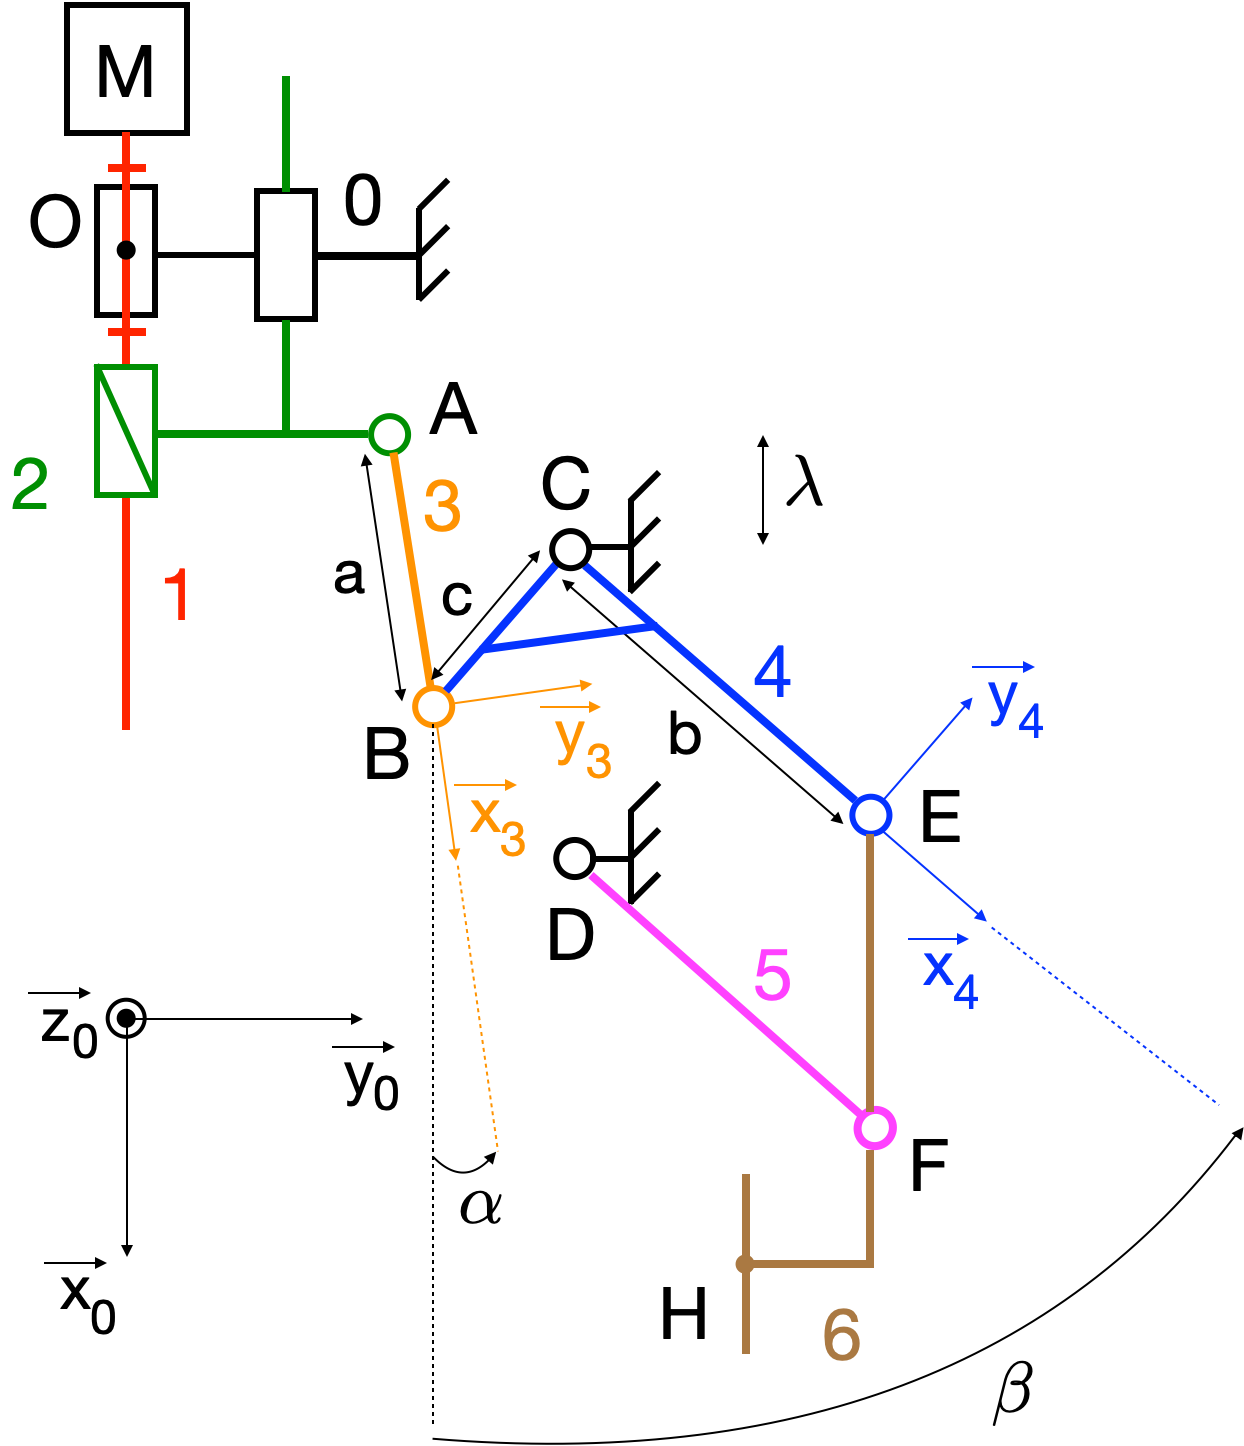
\includegraphics[width=7cm]{fig_01}  & 
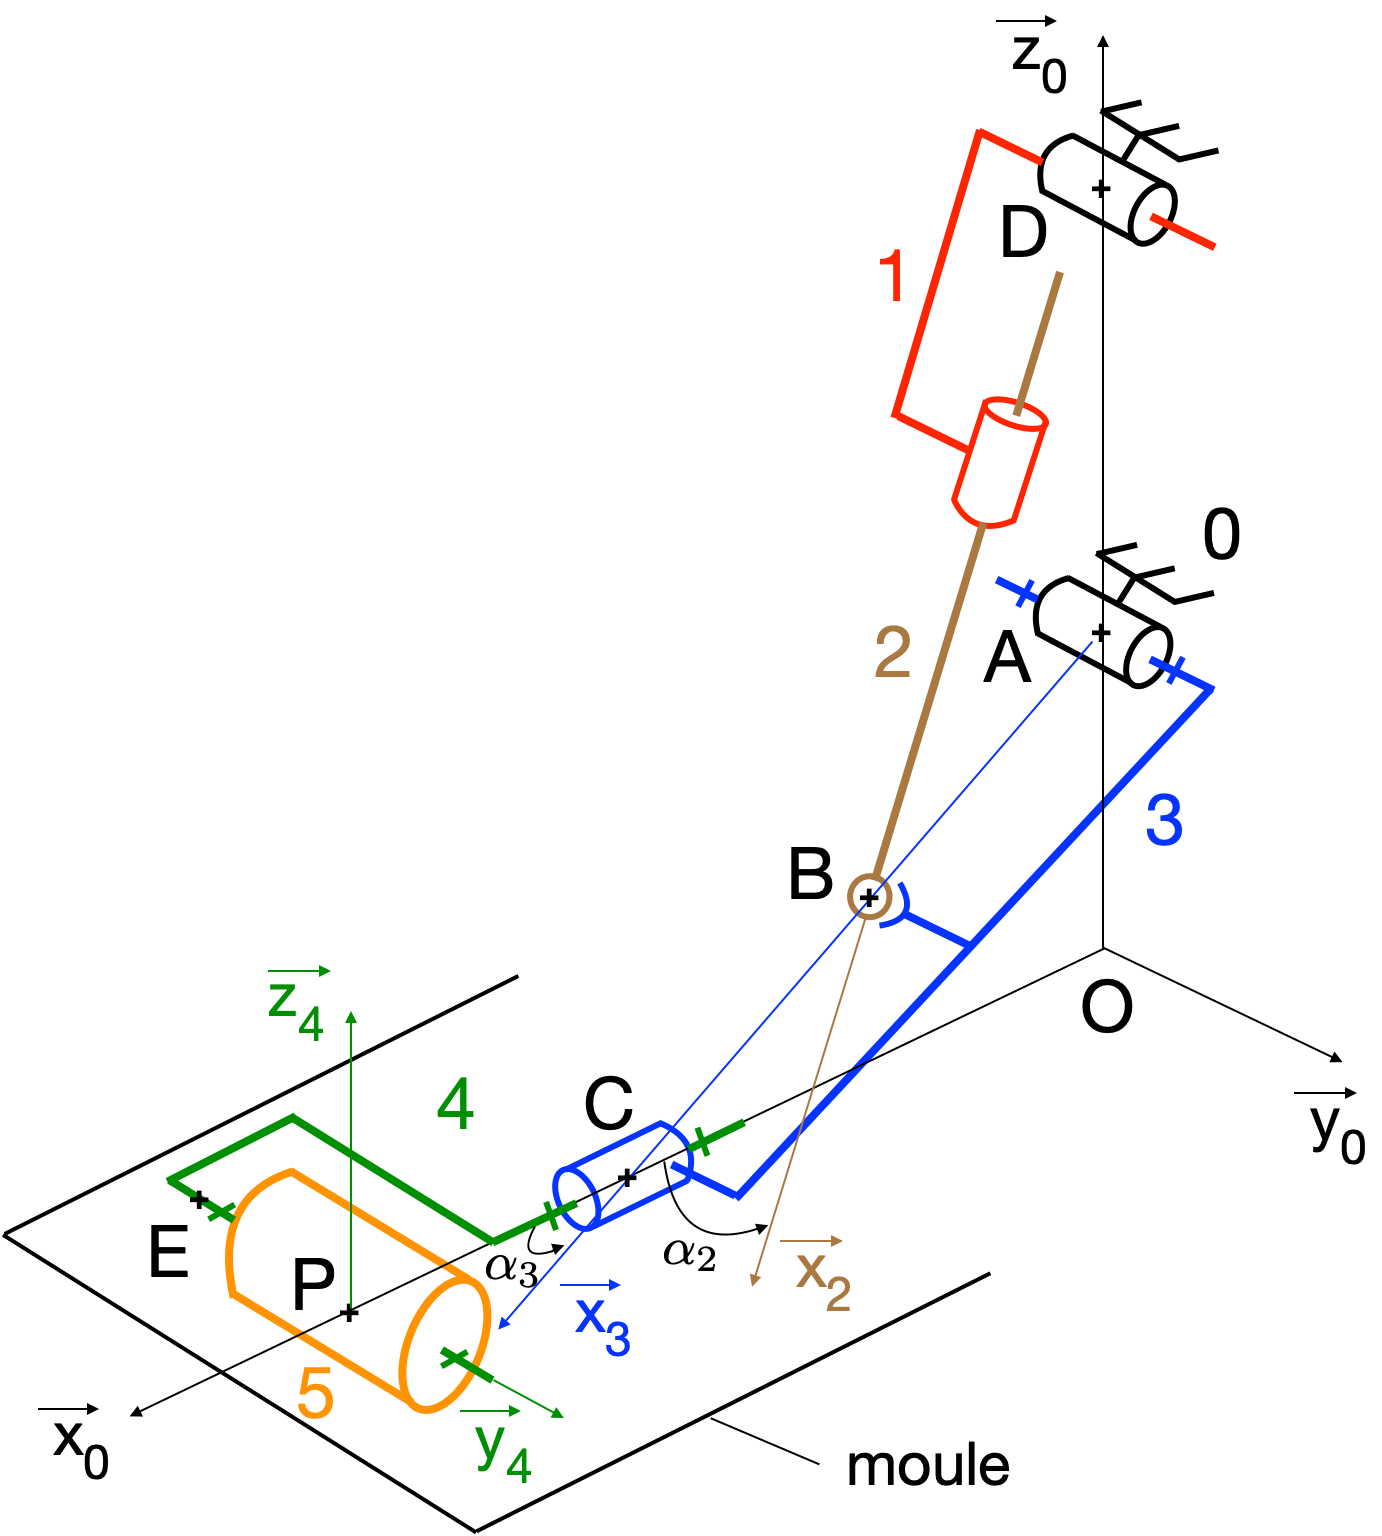
\includegraphics[width=7cm]{fig_03} 
\end{tabular}
\end{center}

\vspace{1cm}

\begin{center}
%\begin{tabular}{cc}
\textbf{Modèle 3 et 3 bis}  \\ %& \textbf{Modèles  4} \\
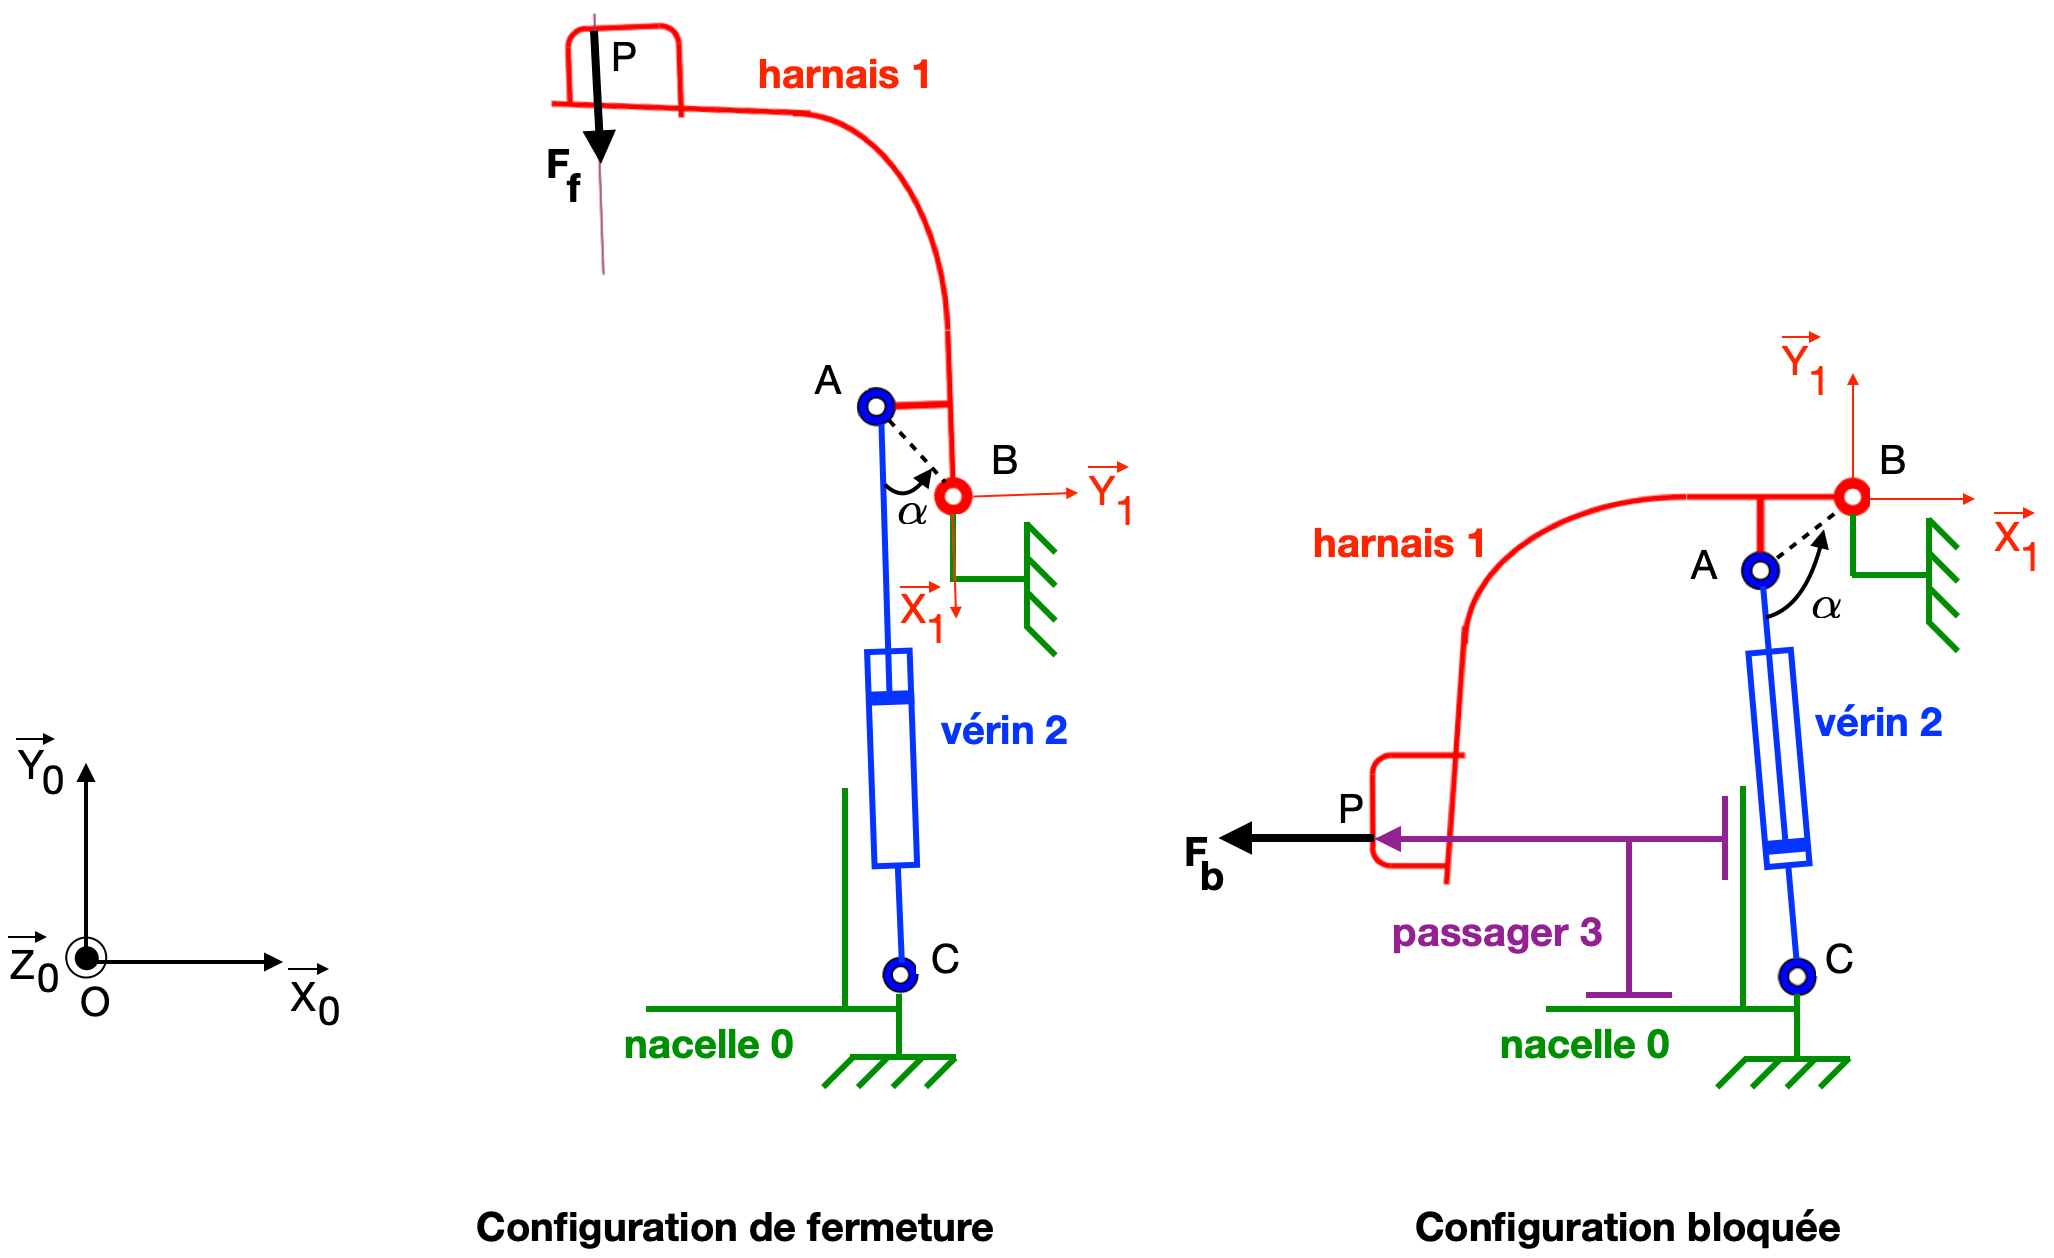
\includegraphics[width=10cm]{fig_02} % & 
%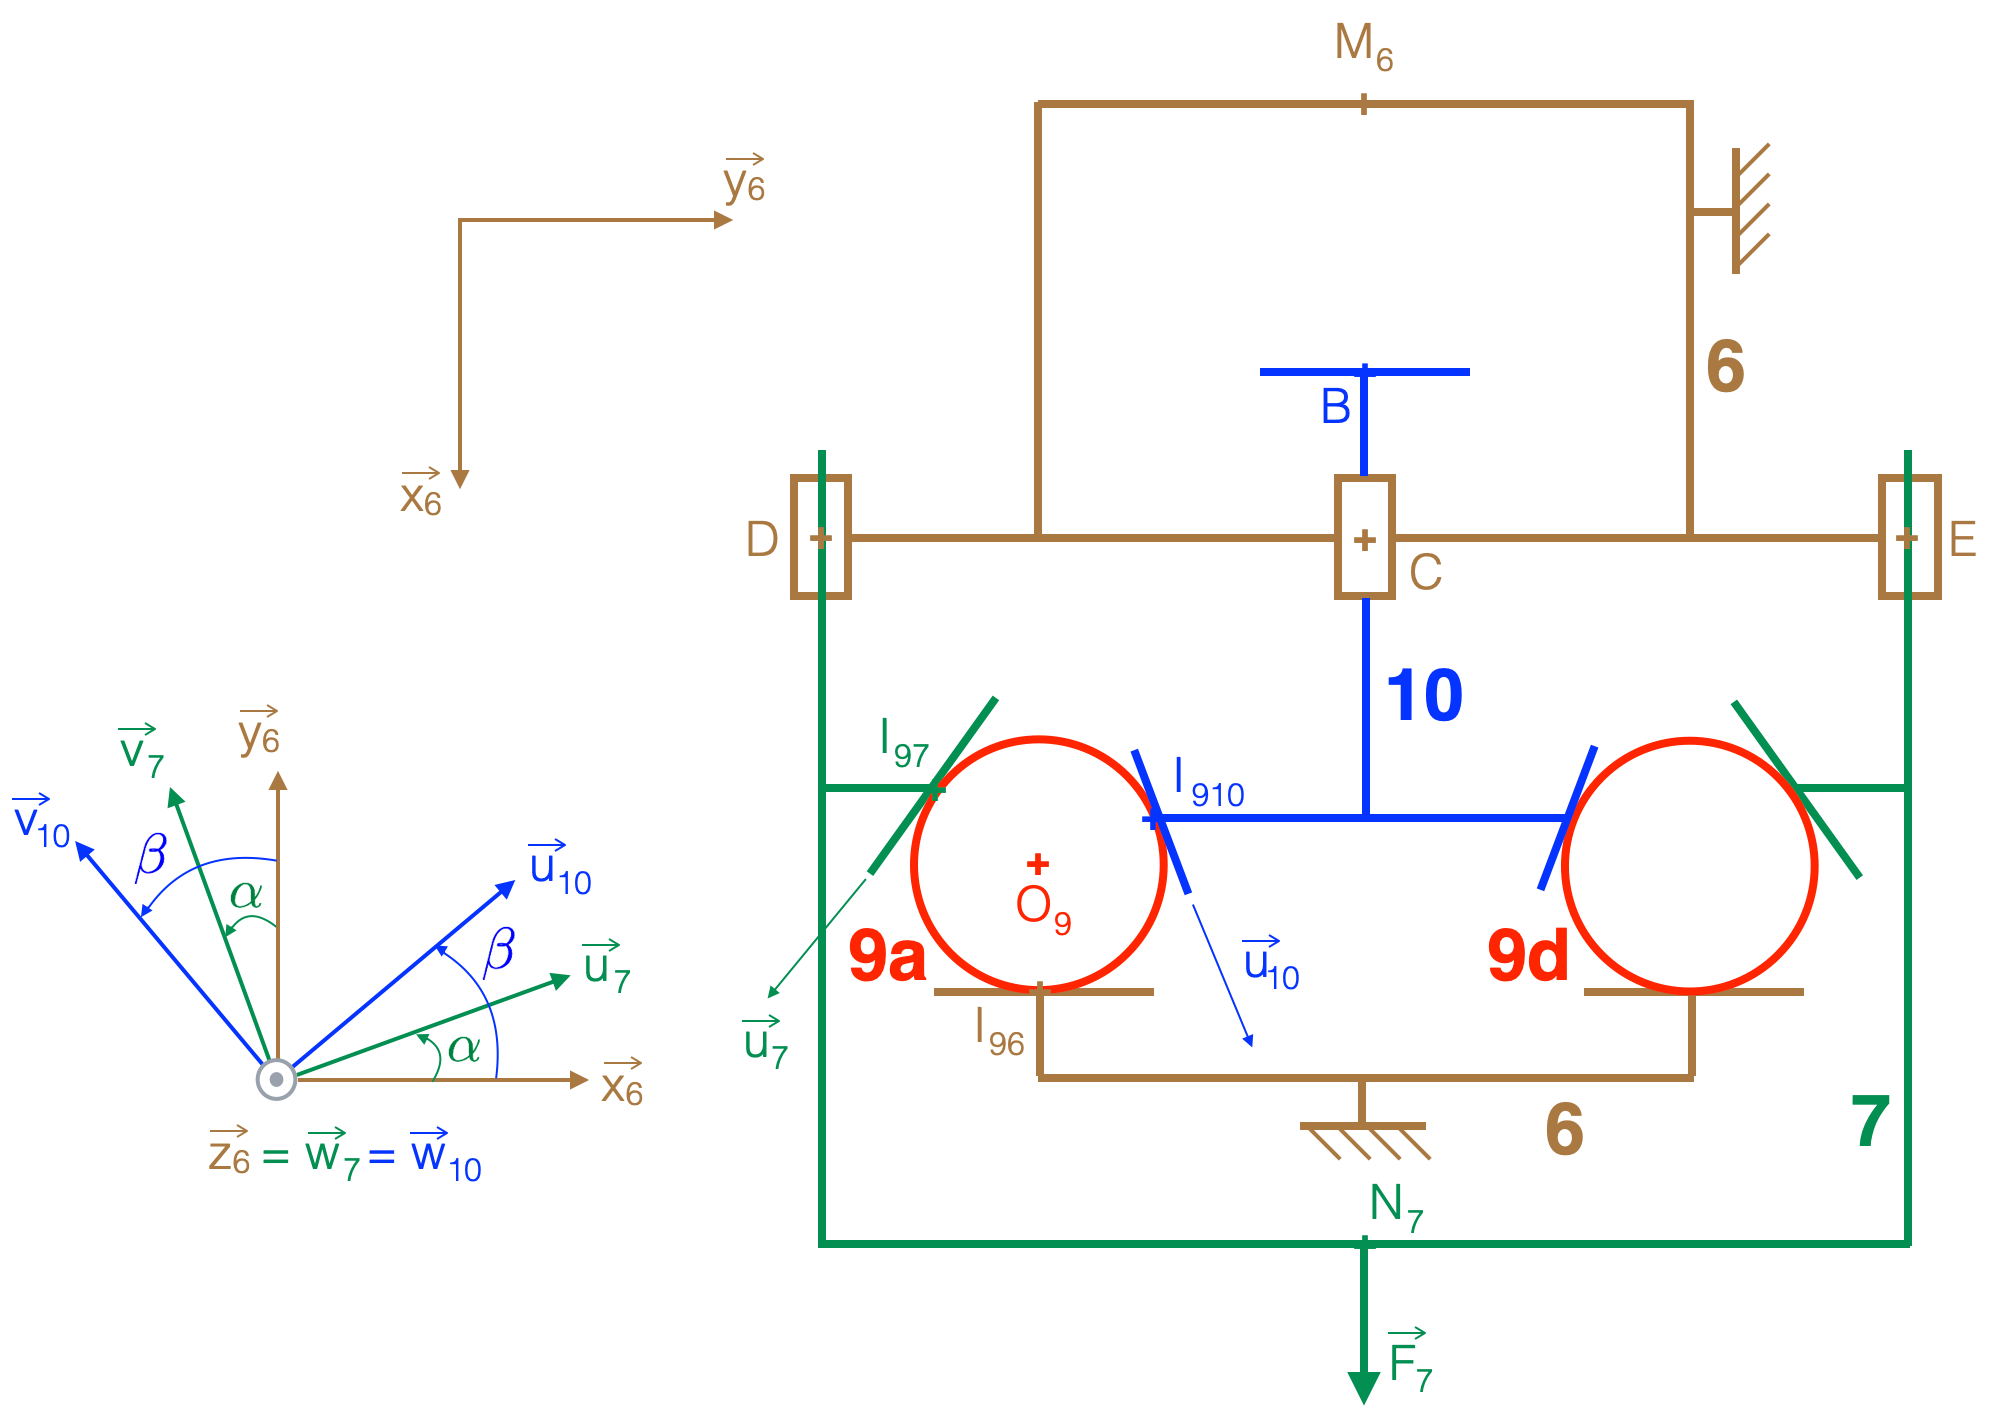
\includegraphics[width=8cm]{fig_04} 
%\end{tabular}
\end{center}

\begin{center}
\begin{tabular}{m{8cm}m{8cm}}
\textbf{Modèle 4}  & \textbf{Modèles  5} \\
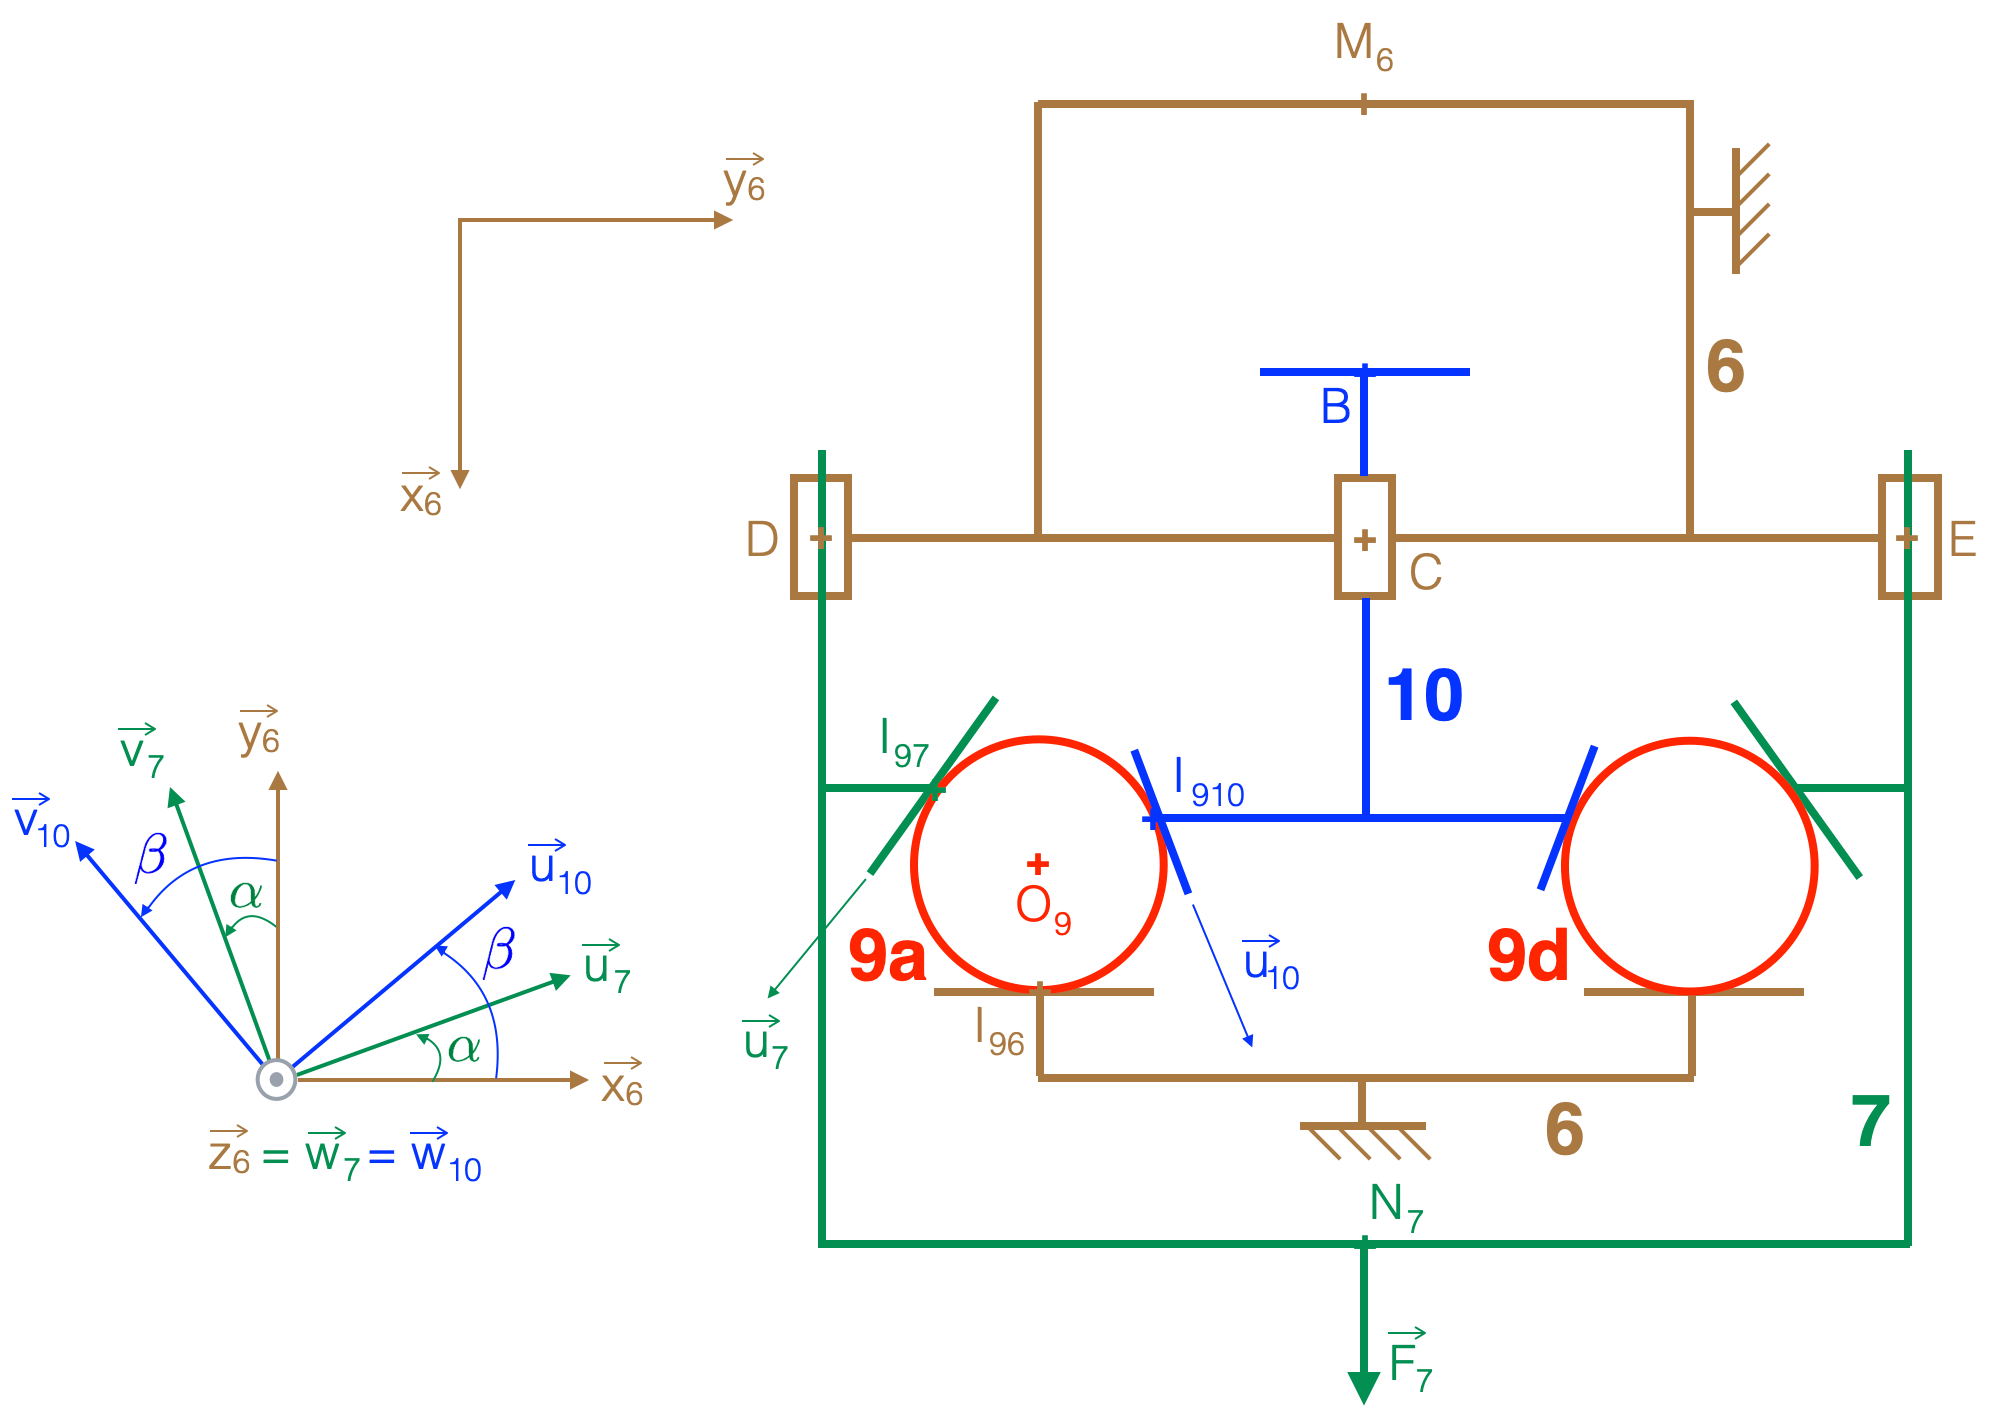
\includegraphics[width=8cm]{fig_04}  & 
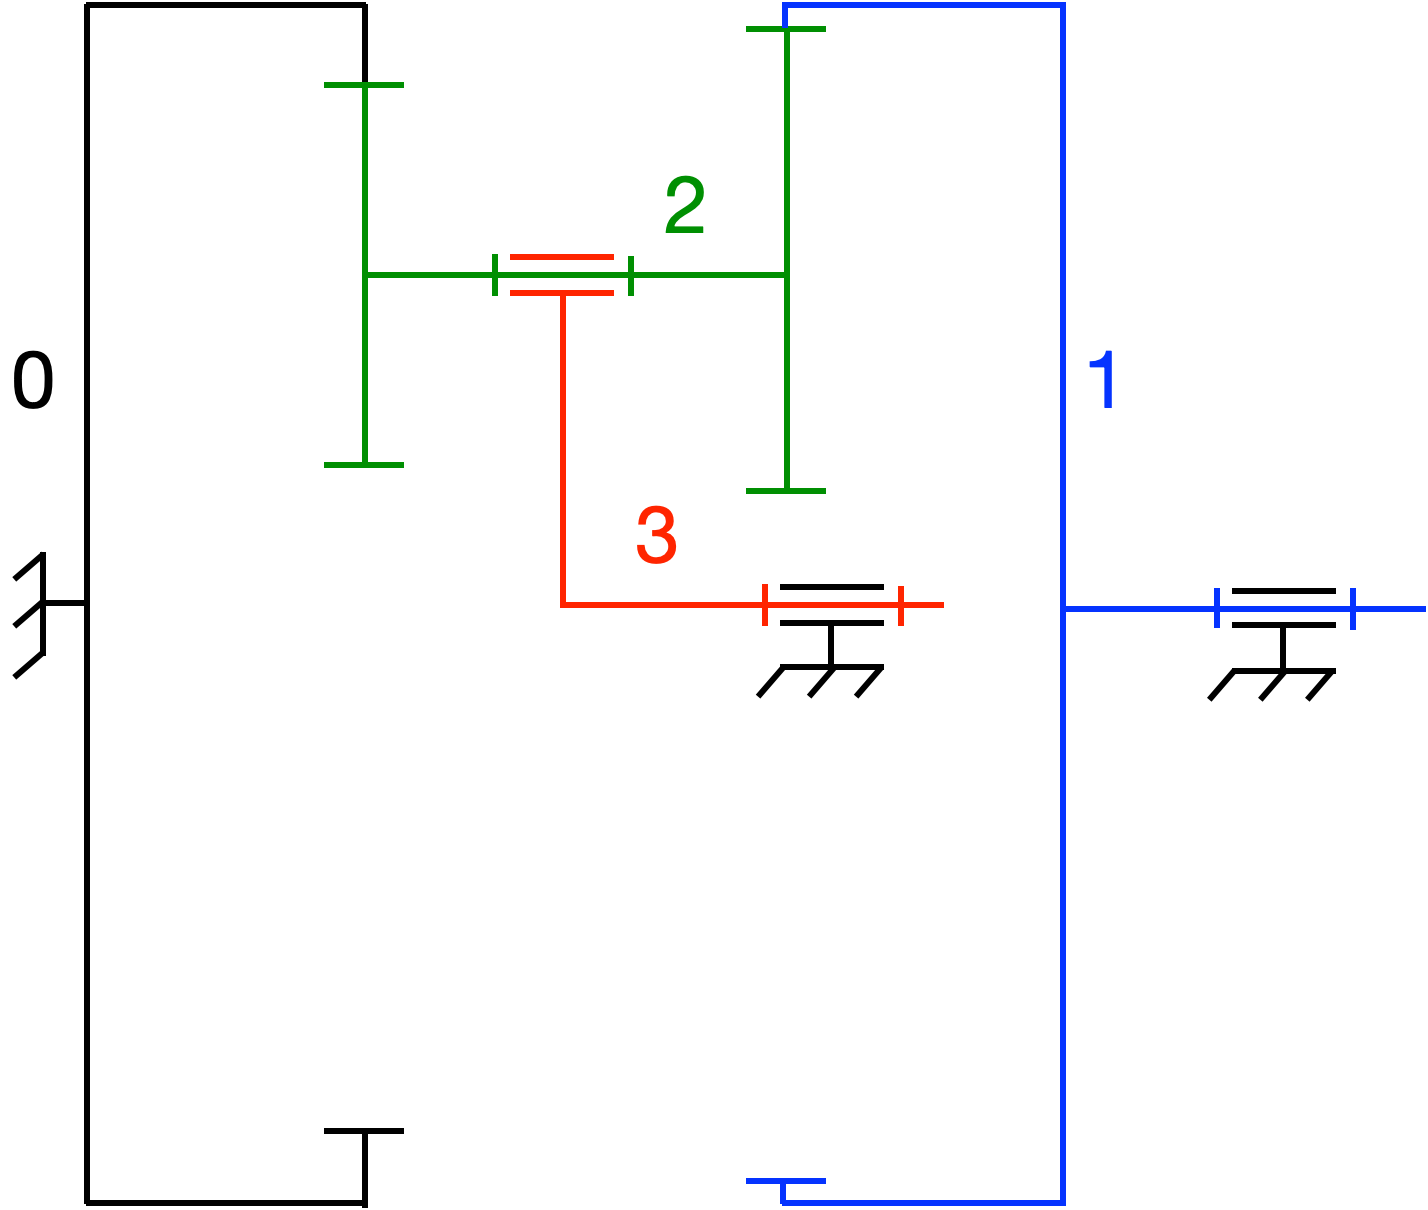
\includegraphics[width=7cm]{fig_05} 
\end{tabular}
\end{center}





\begin{center}
\begin{tabular}{m{8cm}m{8cm}}
\textbf{Modèle 6}  &  \\
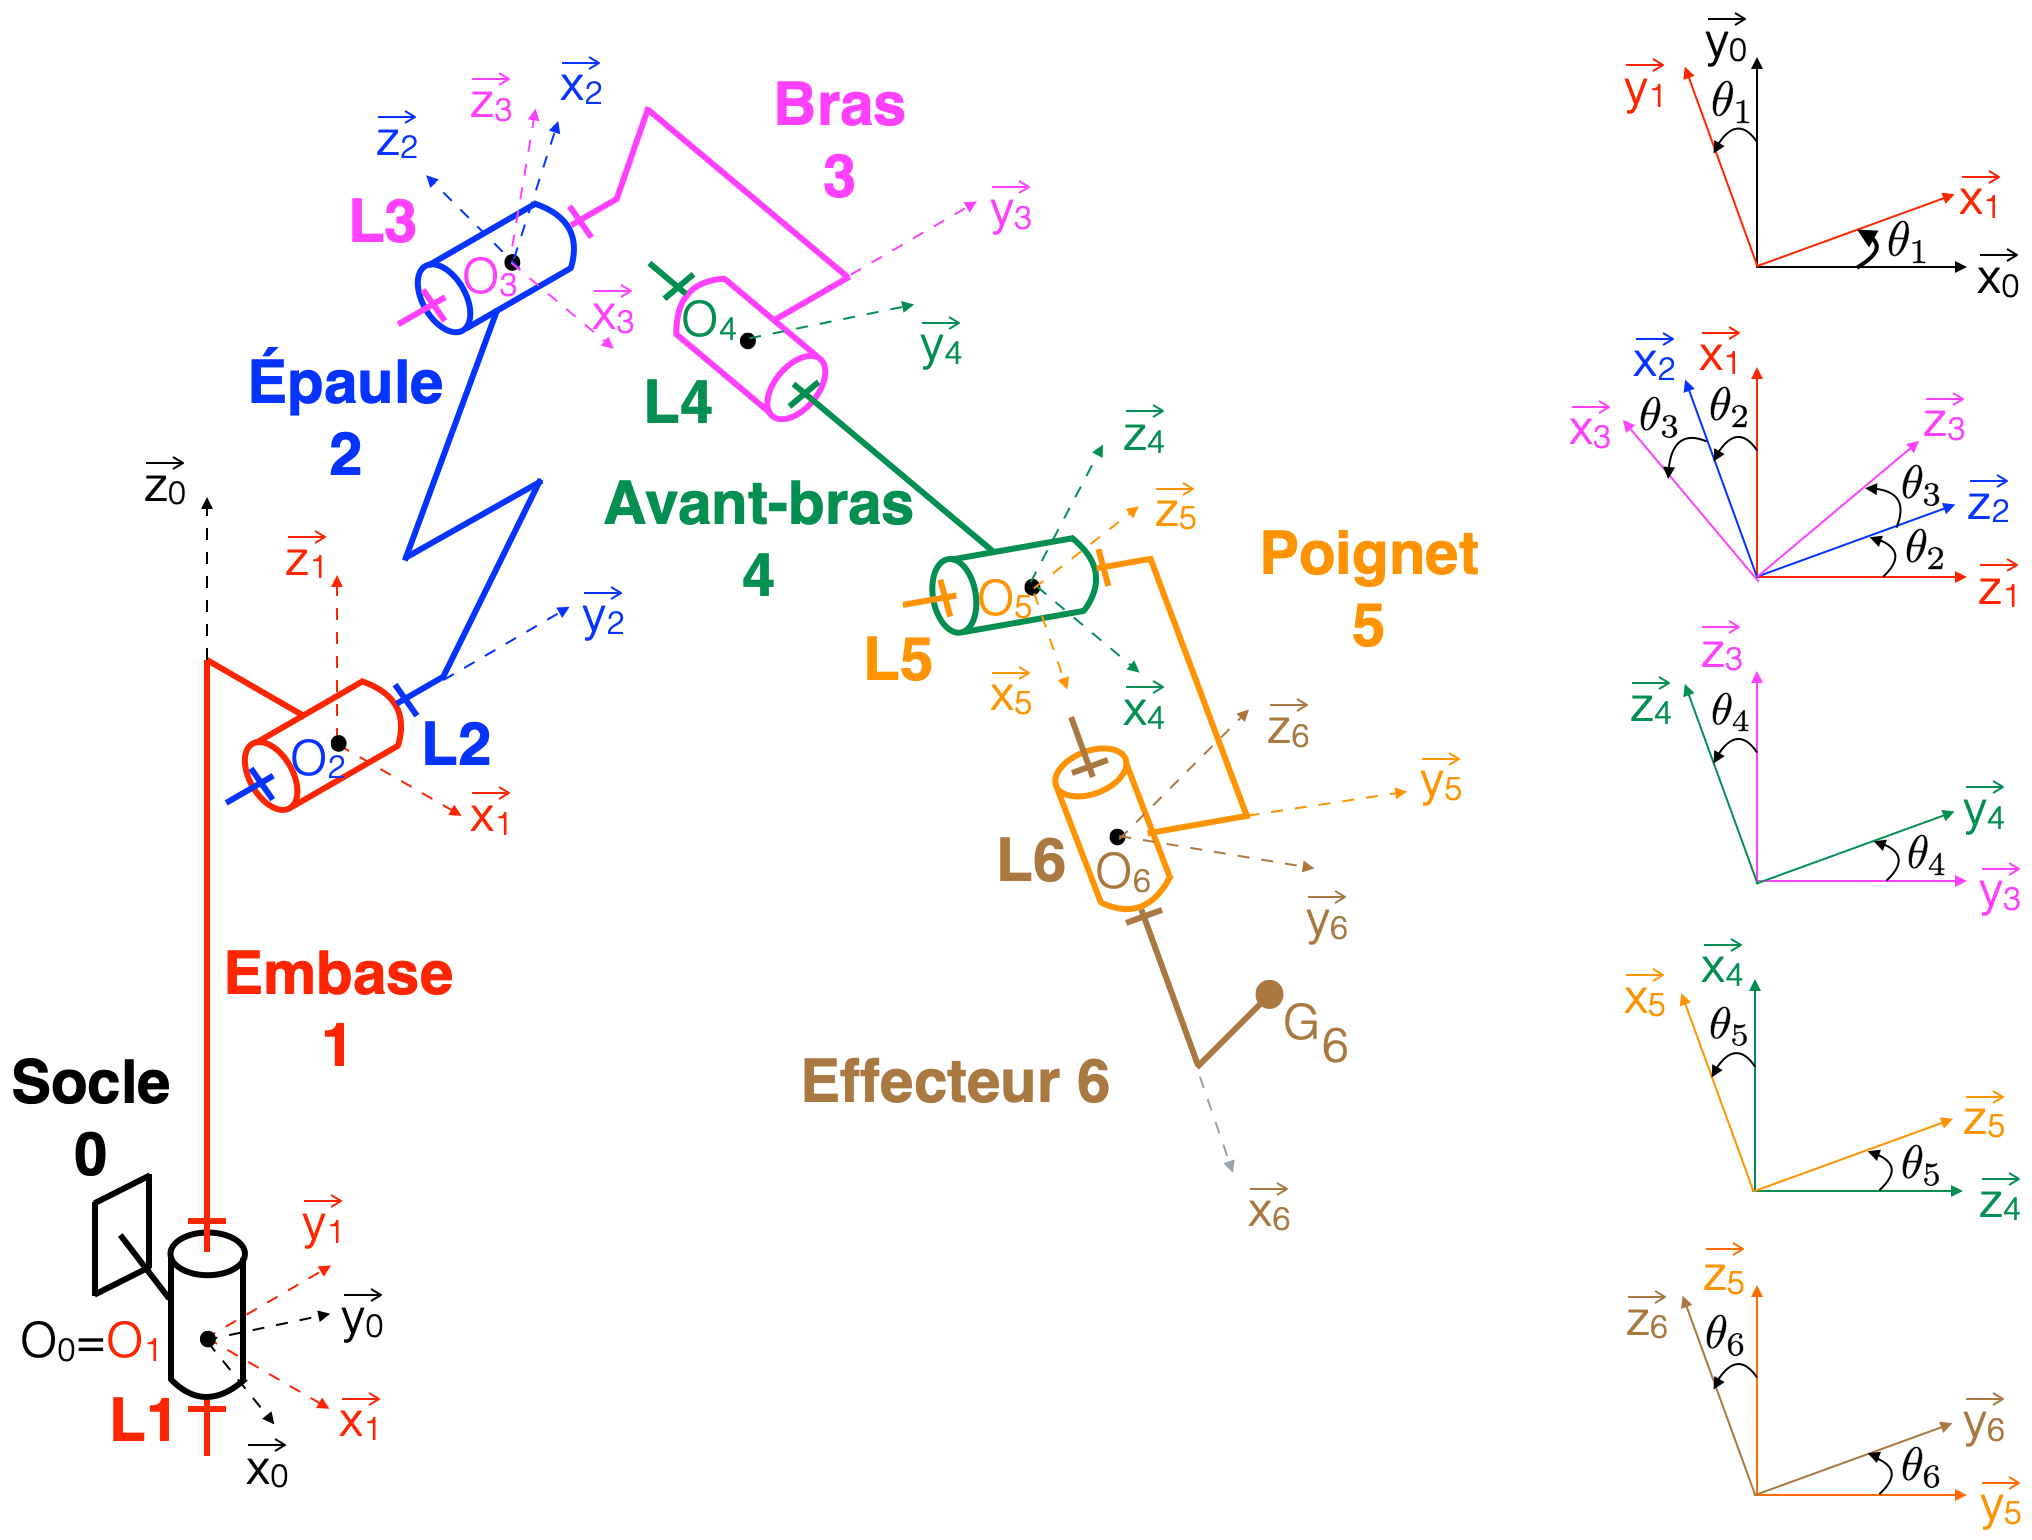
\includegraphics[width=8cm]{fig_07}  & 
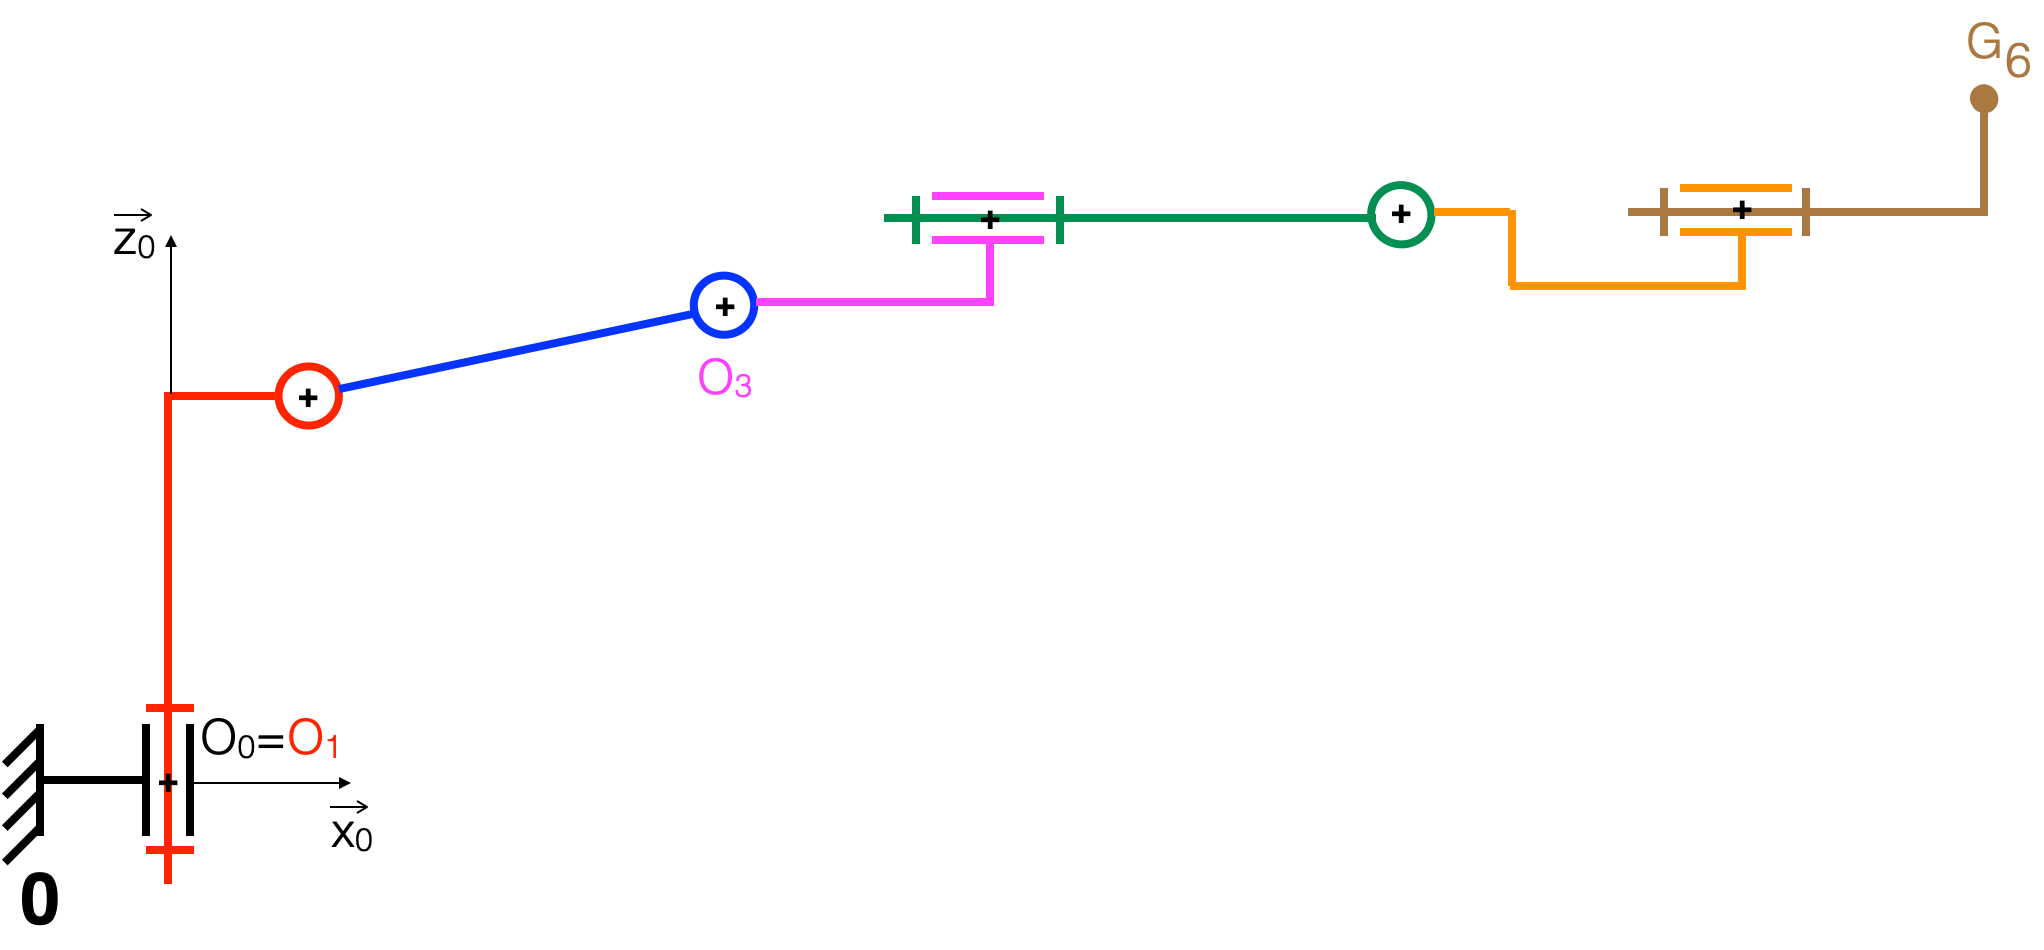
\includegraphics[width=8cm]{fig_06	} 
\end{tabular}
\end{center}



\begin{center}
\begin{tabular}{m{8cm}m{8cm}}
\textbf{Modèle 8}  &  \textbf{Modèle 9}\\
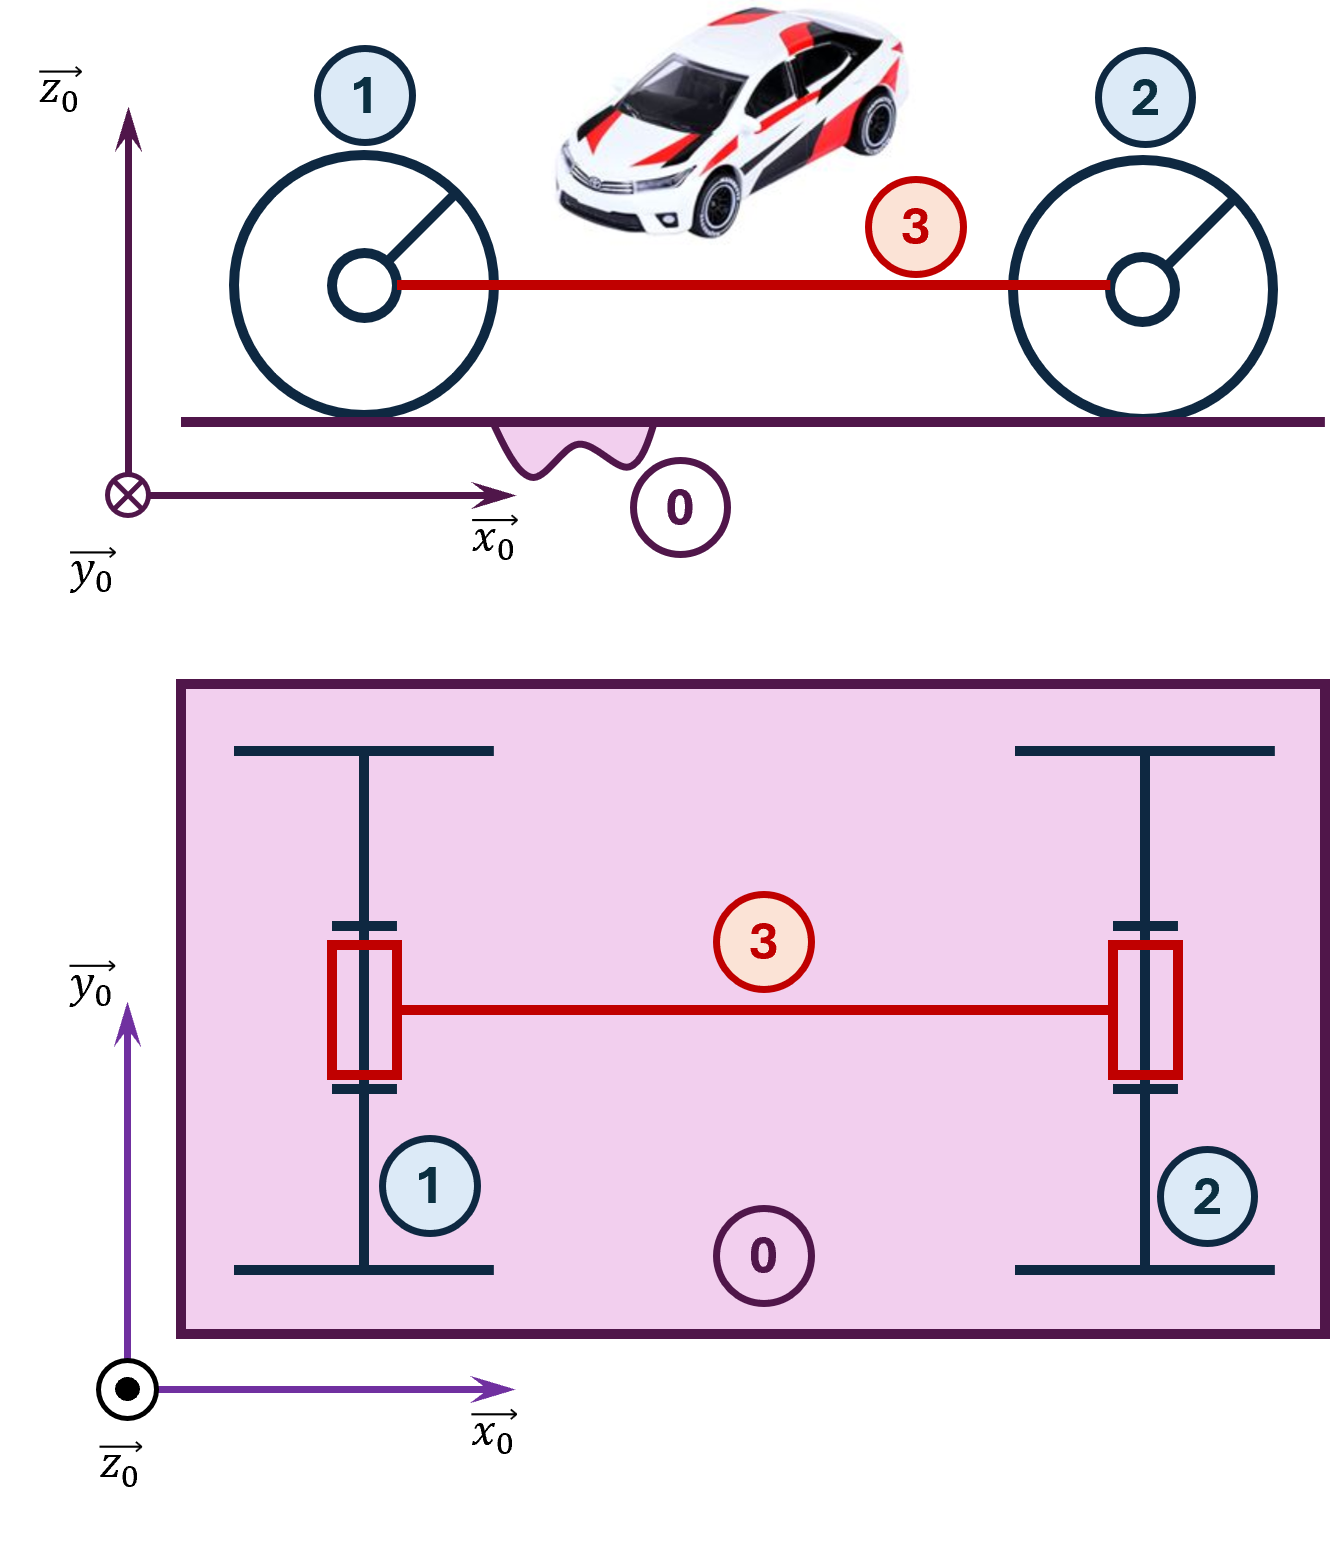
\includegraphics[width=7cm]{fig_08}  & 
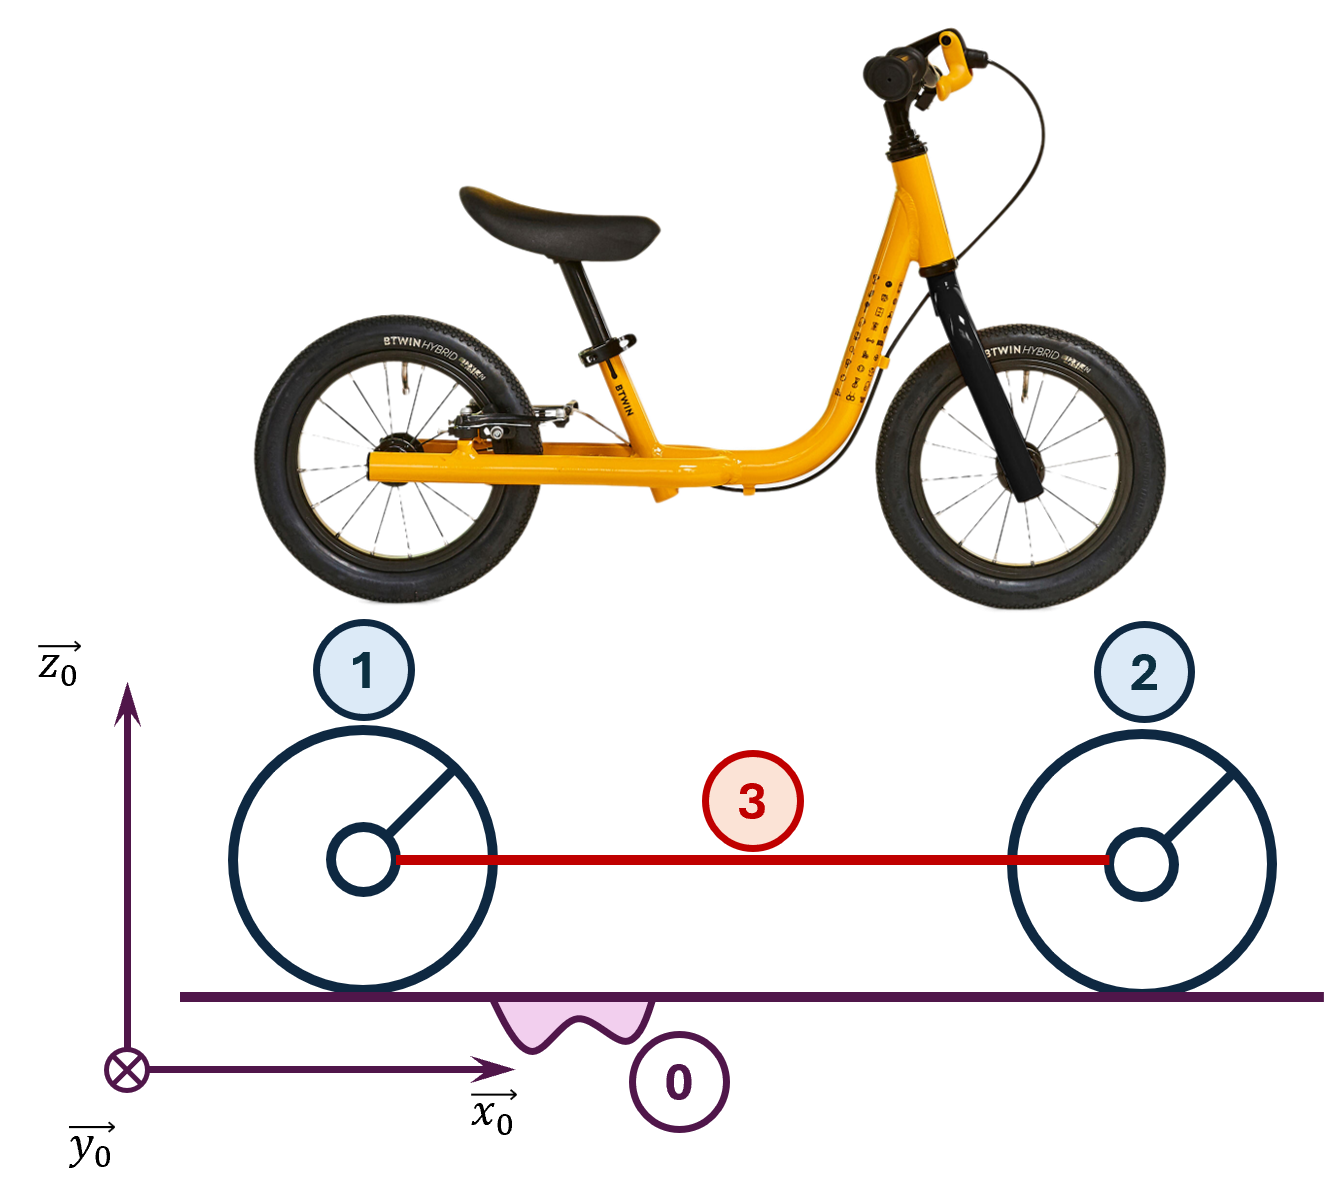
\includegraphics[width=8cm]{fig_09} 
\end{tabular}
\end{center}



\end{document}

